\documentclass[dvipdfmx]{jsarticle}

\usepackage[version=3]{mhchem}
\usepackage{amsmath}
\usepackage[siunitx]{circuitikz}
\usepackage{graphicx}
\usepackage{here}

\setlength\parindent{0pt}

\begin{document}
\title{16 半導体デバイスキャリア統計と電子輸送現象  総合報告書}
\author{電子情報工学科 03-190449 堀 紡希}
\date{\ 10月26日}
\maketitle


\section{抄録}
半導体のキャリアの振る舞いを、代表的なデバイスにおける電子電動現象とホール効果の測定を通じて体感することで、半導体物性と電子デバイスについて理解する。
\section{目的}
半導体のキャリアの振る舞いを、代表的なデバイスにおける電子電動現象とホール効果の測定を通じて体感することで、半導体物性と電子デバイスについて理解する。実験結果を理論と比較検討することにより、半導体のキャリア統計と電子伝導の現象の基礎を学ぶ。
\section{実験}

\subsection{原理}
ホール効果の概要を図1に示す。
\begin{figure}[H]
\begin{center}
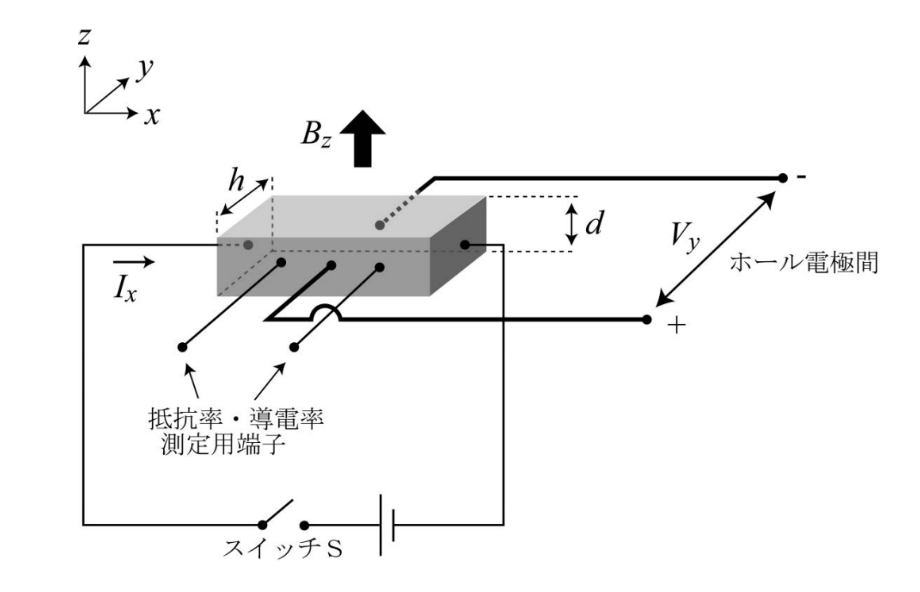
\includegraphics[scale = 0.6]{figure1.png}
\caption{ホール効果の測定}
\end{center}
\end{figure}

図のように$x,y,z$軸をそれぞれ定めると、厚さ$d$(m)の試料に電流$I_{x}$(A),磁束密度$B_{z}$(T)をかけたとき、ホール電圧$V_{y}$(V)が
\begin{equation}
V_{y} = R_{H}\frac{I_{x}B_{z}}{d}
\end{equation}
生じる。ここで$R_{H}$は試料によって定まるホール係数である。

図1において、試料がp型半導体と仮定して、ドリフト速度$v_{x}$で移動すると仮定すると正孔が受けるローレンツ力は正孔の電荷を$q$として、
\begin{equation}
F_{y} = -qv_{x}B_{z}
\end{equation}
と表される。
定常状態において、ローレンツ力と、密度勾配によって生じる電界が釣り合うので、$qE_{y} = qv_{x}B_{z}$が成り立つから、正孔の密度をp[1/cm$^{3}$]とすると、$I_{x} = pqv_{x}hd$より
\begin{align}
V_{y} &= E_{y}h\\
&= v_{x}B_{z}h\\
&= \frac{1}{pq}\frac{I_{x}B_{z}}{d}
\end{align}
となる。
(1)と比較して、
\begin{equation}
R_{H} = \frac{1}{pq}
\end{equation}
である。

n型の場合は、$p = -n$とすればそのまま成り立つ。

しかし、本実験では半導体がボルツマン分布に従い、電子や正孔が熱散乱を受けると考え、
\begin{equation}
R_{H} = \frac{3\pi}{8pq}, -\frac{3\pi}{8nq}
\end{equation}
とする。

ホール効果の測定から測定試料のキャリア濃度と移動度を求めるために、パウ法(後述)で電導率$\sigma$を求め、p型半導体の場合は、
\begin{equation}
p = \frac{3 \pi }{8}\frac{1}{qR_{H}}
\end{equation}
\begin{equation}
\mu _{p} = \frac{8}{3 \pi} \sigma R_{H}
\end{equation}
と求められる。(n型も同様)


次にパウ法によって試料の抵抗率、ホール係数を測定する方法を紹介する。
\begin{figure}[H]
\begin{center}
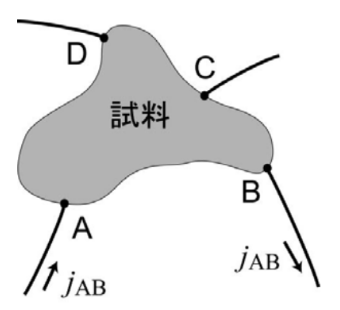
\includegraphics[scale = 0.6]{figure2.png}
\caption{パウ法による測定}
\end{center}
\end{figure}
試料の厚さが均一のとき、図2のようにサイクリックに電極を配置し(電極の位置は任意)電極Aから電極Bに電流$j_{AB}$を流したときに、電極C,D間に生じる電位差を$V_{D}-V_{C}$とする。$R_{\rm{AB} \cdot \rm{CD}}$を
\begin{equation}
R_{\rm{AB} \cdot \rm{CD}} = \frac{V_{D}-V_{C}}{j_{AB}}
\end{equation}
と定義すると、抵抗率$\rho$は
\begin{equation}
\rho = \frac{\pi d}{\rm{ln}2}\frac{R_{\rm{AB} \cdot \rm{CD}} + R_{\rm{BC} \cdot \rm{DA}}}{2}f\left(\frac{R_{\rm{AB} \cdot \rm{CD}}}{R_{\rm{BC} \cdot \rm{DA}}}\right)
\end{equation}
と表せる。
ただし$f$は
\begin{equation}
\frac{R_{\rm{AB} \cdot \rm{CD}} + R_{\rm{BC} \cdot \rm{DA}}}{R_{\rm{AB} \cdot \rm{CD}} - R_{\rm{BC} \cdot \rm{DA}}} = \frac{f}{\rm{ln}2}\left(\cosh^{-1}\frac{exp(\rm{ln}2/f)}{2}\right)
\end{equation}
を満たす。


またホール係数は試料に垂直に磁場Bをかけたときの$R_{AC\cdot BD}$の変化を$\Delta R_{\rm{AC}\cdot \rm{BD}}$とすると、
\begin{equation}
R_{\rm{H}} = \frac{d}{B}\cdot \Delta R_{\rm{AC}\cdot \rm{BD}}
\end{equation}
移動度は
\begin{equation}
\mu = \frac{d}{B}\cdot \frac{\Delta R_{\rm{AC}\cdot \rm{BD}}}{\rho}
\end{equation}
と表される。
\subsection{方法}
\subsubsection{実験(1) 室温}
実験班5人の中で2グループに分かれ、Ge, 厚さが異なるSi, GaAs試料のそれぞれについて、電流$I_{\rm{x}}$を流し、室温における導電率をパウ法を使って求め、次に磁場$B_{\rm{z}}$を変化させながらかけて、ホール電圧を測定することでホール係数を求め、さらにそこから、キャリア密度、ホール移動度計算する。

また、ホール係数の符号から試料の導電型を判定する。


\subsubsection{実験(2) 温度変化}
室温で行った実験をクライオスタット、液体窒素を用いて温度を変えながら行うことで、移動度、キャリア密度の変化を求める。

具体的には-196℃から0℃まで7点、30℃から130℃まで7点測定する。


\subsubsection{実験 異常ホール効果}

強磁性半導体であるGaMnAsを4Kから100Kまでの間で-500Gから500Gの磁場の間でホール効果を測定することで異常ホール効果を観測する。

なお本実験はプログラムを用いて測定する。
\section{結果}

\section{考察}
\subsection*{(1) 移動度}
移動度は、電界$E$中の、キャリアの平均速度$<v>$を用いて
\begin{equation}
\mu = \frac{<v>}{E}
\end{equation}
と定義される。

移動度を測定することにより、キャリアの結晶中での移動するときの通りやすさがわかる。
\subsection*{(2) 移動度の性質}
同種の半導体で、不純物濃度が同じなら、n型の方が移動度が大きい。
なぜなら、キャリアの電荷$q$と有効質量$m^{\ast}$に対し(15)式と等価な式
\begin{equation}
\mu = \frac{q\tau}{m^{\ast}}
\end{equation}が成り立ち、正孔より電子の方が有効質量が小さいからである。
\subsection*{(3)}
\subsection*{(4)}
図『後で記入』より、$T = 300$Kほどで真性領域に達している。
\subsection*{(5)}
\subsection*{(7)}
\section{結論}



\section{参考文献}
[1]東京大学工学部:「電気電子情報第一(前期) 実験テキスト」, 2019.

[2]廣瀬明:「電気電子計測」, 数理工学社, 2003.

[3]日高邦彦:「高電圧工学」, 数理工学社, 2013
\end{document}